\section{Appendix}
But, when the planet is not too close to the sun, the integration with $dt=1$ is sufficient for a reasonable accuracy, which is shown in Figure \ref{fig:Planet2AUdt1}:

\begin{figure}[H]
\centering
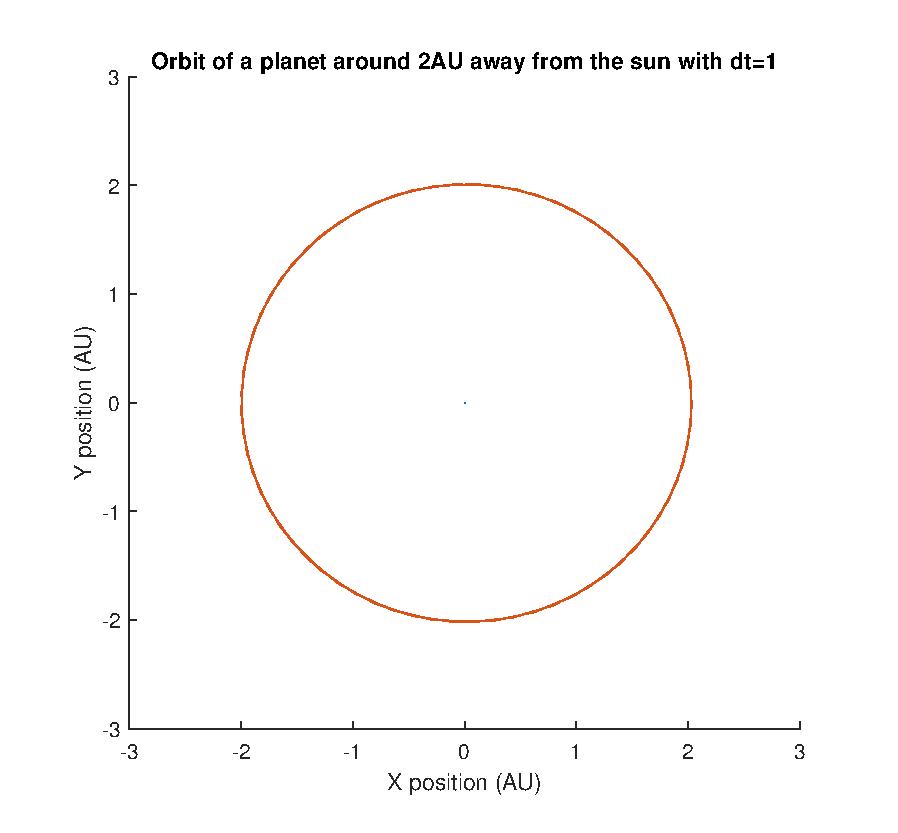
\includegraphics[width=0.6\textwidth]{Planeet_2AU_dt1_10jaar.eps}
\caption{Orbit of a planet of 1 $M_{\oplus}$ with a distance around 2AU from the sun, integrated with $dt=1$ month over $10$ years.}
    \label{fig:Planet2AUdt1}
\end{figure}

Also, the energy calculation (Table \ref{tab:Planet2AUEnergy}) shows that the energy is better conserved:

\begin{table}[htb]
\centering
\caption{The total energy of the system, which consists of a planet rotating around 2AU away from the sun. The energy is calculated after each 20 time steps.}
\begin{tabular}{|l|l|l|l|l|l|l|l|}
\hline
k-th timestep&0&20&40&60&80&100&120\\ \hline
$E_{tot}$&-0.0680&   -0.0658&   -0.0657&   -0.0658&   -0.0658&   -0.0657&   -0.0658\\ \hline
\end{tabular}

\label{tab:Planet2AUEnergy}
\end{table}

And if the planet is quite far from the sun, like around 5AU, then the energy is very well conserved and the orbit is also quite smooth:

\begin{figure}[H]
\centering
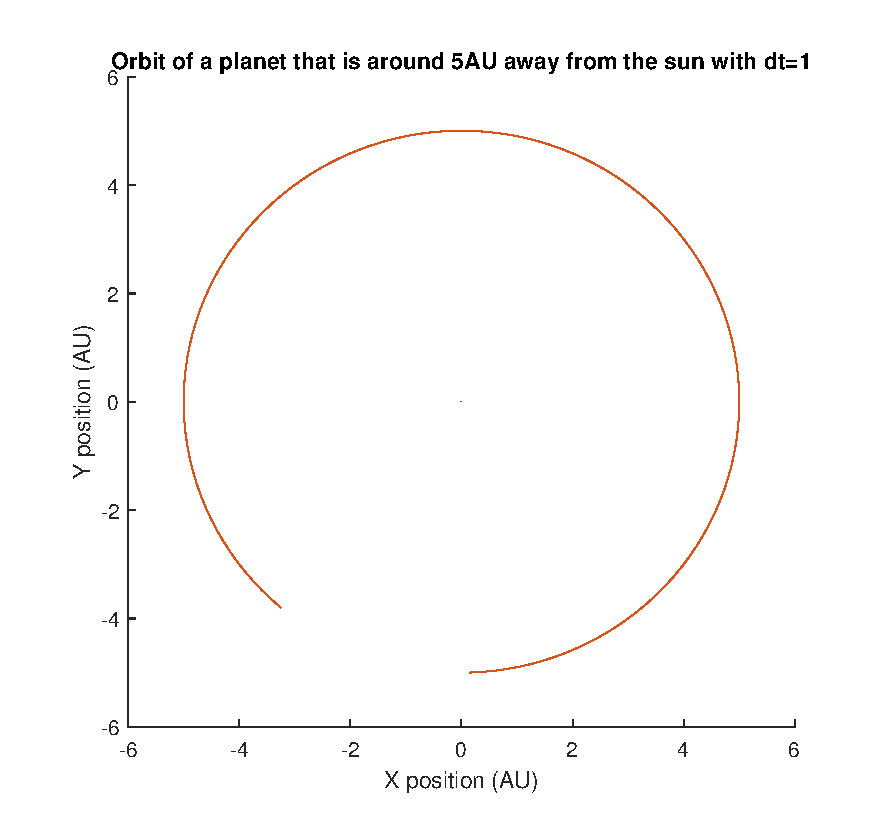
\includegraphics[width=0.6\textwidth]{Planeet_5AU_dt1_10jaar.eps}
\caption{Orbit of a planet of 1 $M_{\oplus}$ with a distance around 5AU from the sun, integrated with $dt=1$ month over $10$ years. Apparently, this planet has an orbital period longer than 10 years.}
    \label{fig:Planet5AUdt1}
\end{figure}

\begin{table}[htb]
\centering
\caption{The total energy of the system, which consists of a planet rotating around 5AU away from the sun. The energy is calculated after each 20 time steps.}
\begin{tabular}{|l|l|l|l|l|l|l|l|}
\hline
k-th timestep&0&20&40&60&80&100&120\\ \hline
$E_{tot}$&-0.0272&   -0.0271&   -0.0271&   -0.0271&   -0.0271&   -0.0271&   -0.0271\\ \hline
\end{tabular}
\label{tab:Planet5AUEnergy}
\end{table}